% !TEX root =  master.tex 
\chapter{Bereinigung von Fehlern -- Manuel Techert}

Gegen Ende des Projekts wollen wir die Qualität unseres Projektes noch einmal erhöhen und etwaigen Fehlern vorbeugen.

Dazu nutzen wir die Plattform SonarQube, die uns bei einem Verstoß gegen unsere definierten Regeln mitteilt, wo nachgebssert werden sollte. 

Um einen aktuellen Stand unsere Regelverstöße zu haben, führe ich eine Analyse mit dem Scanner von SonarQube zu, dessen Ergebnisse im Web-Server abgelegt werden (siehe nachfolgende Abbildung).
\\

\begin{minipage}{\linewidth}
	\centering 
	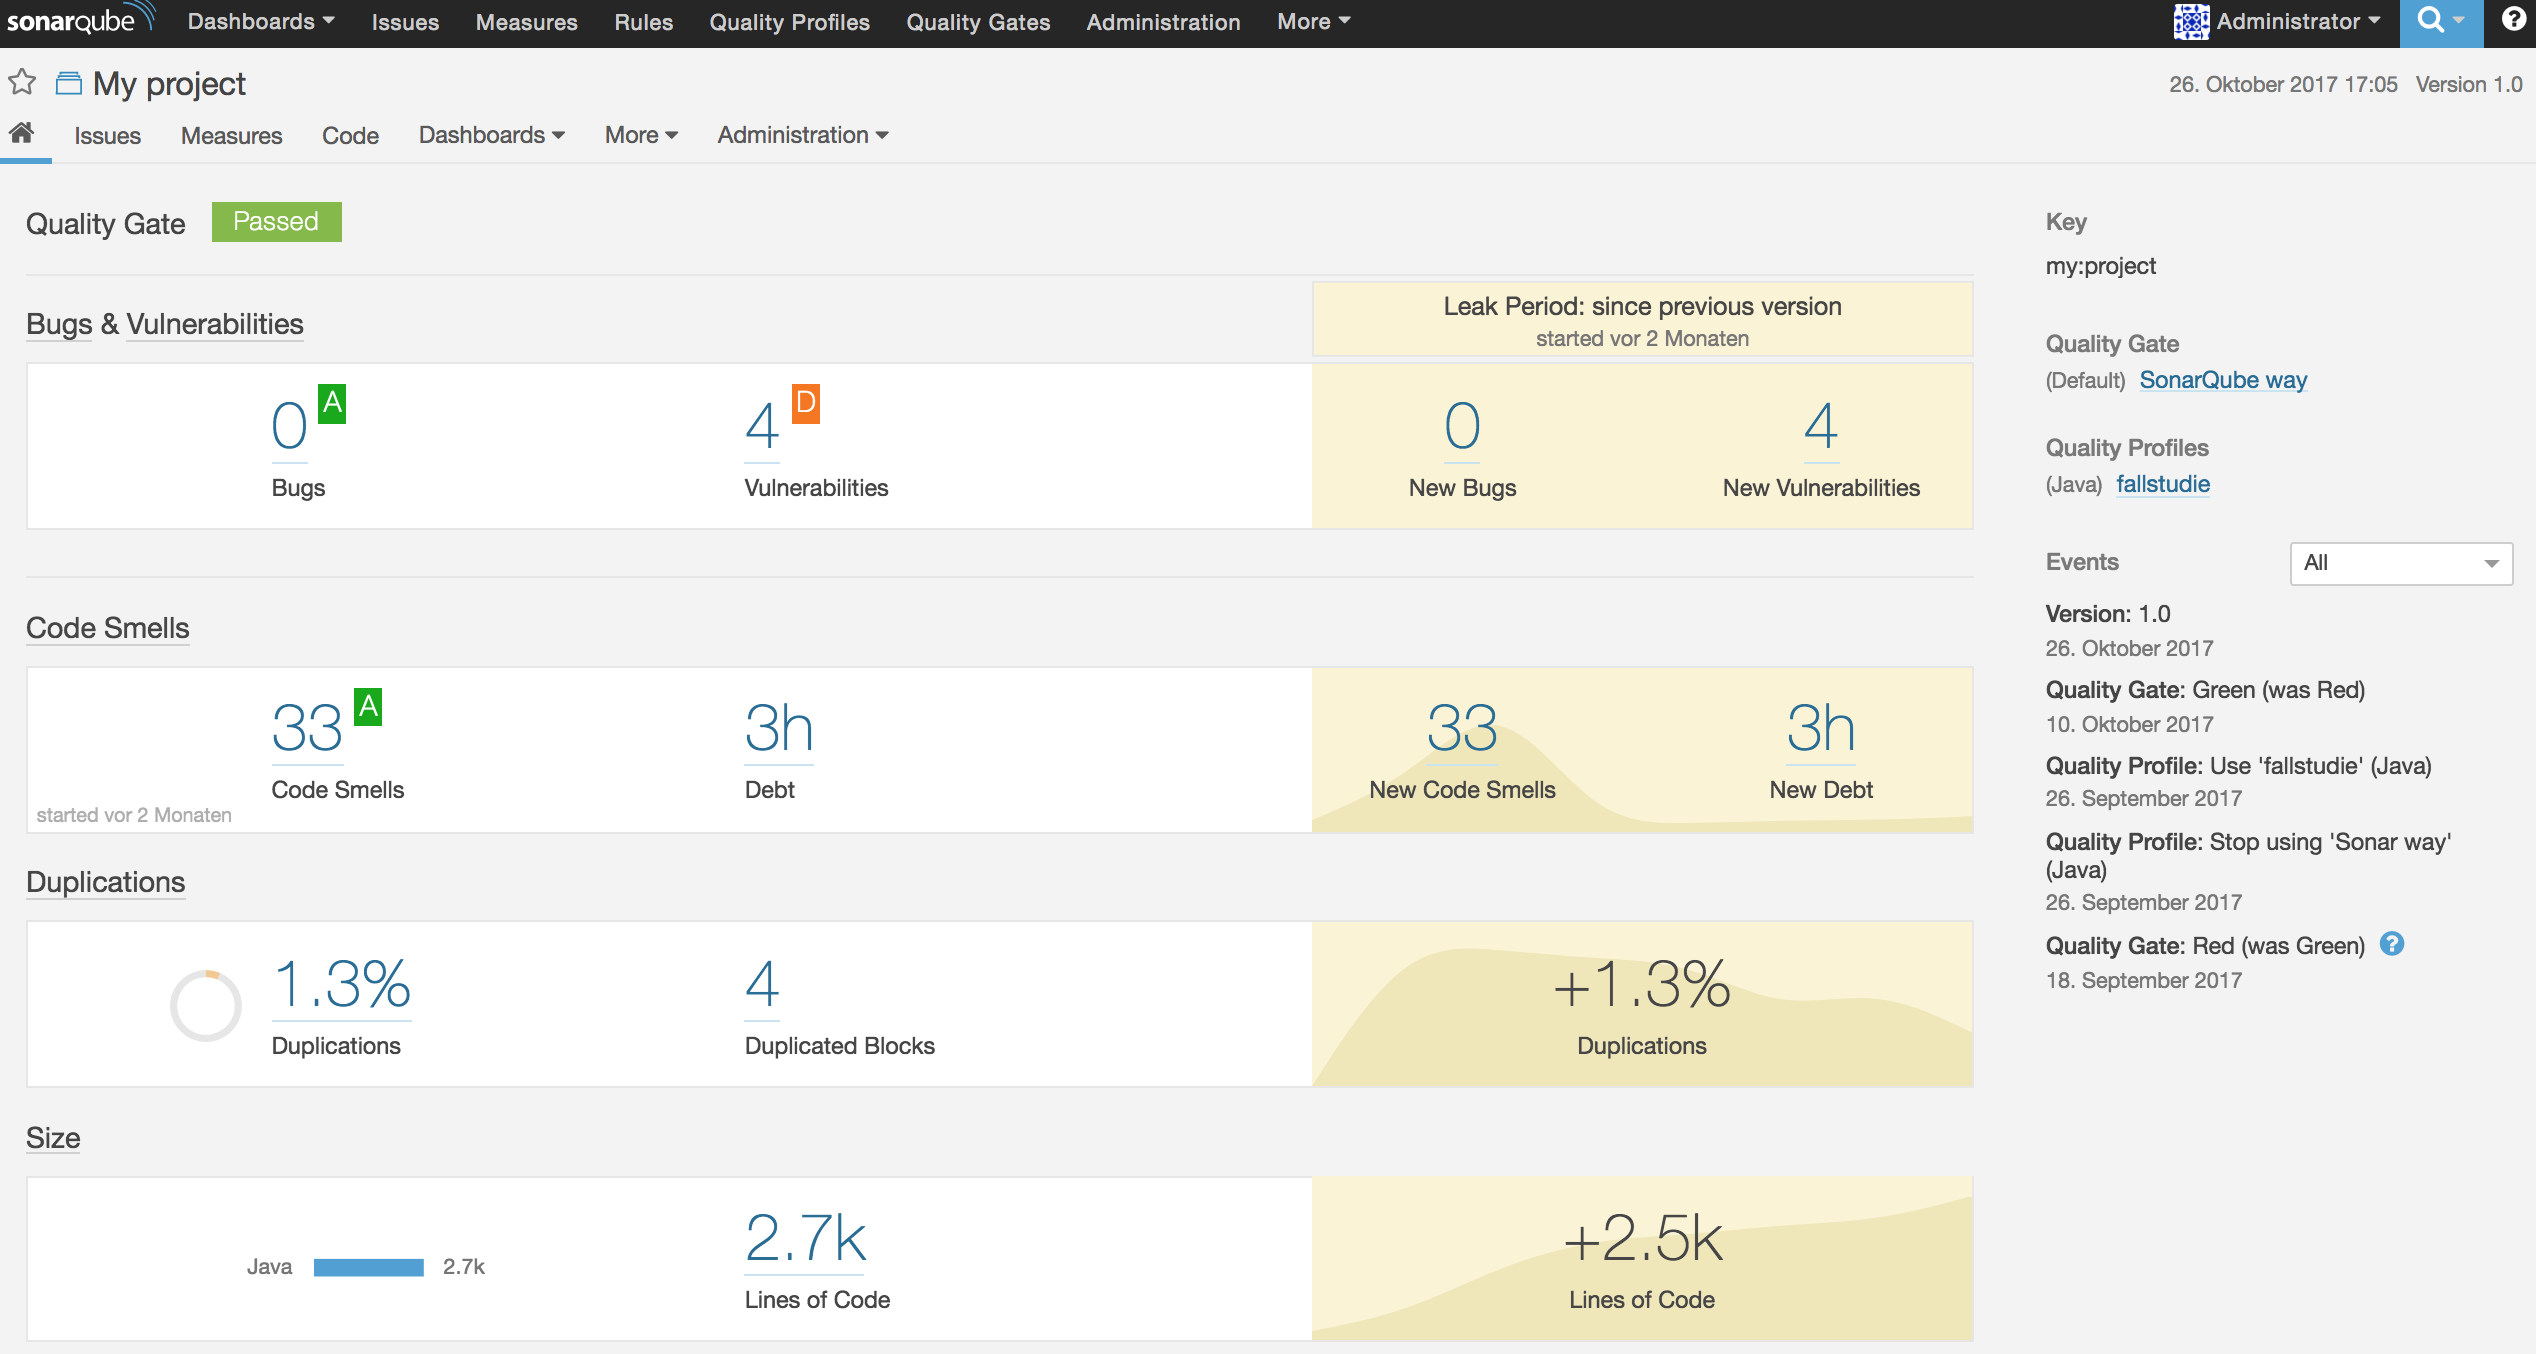
\includegraphics[scale=0.35]{img/startSonar}
	\captionof{figure}{\label{abb:startsonar}Die Startseite des SonarQube-Servers.}
	\vspace{2em}
\end{minipage}

Bei Einsicht der Ergebnisse sehen wir, dass wir an einigen Stellen Strings mit einem doppelten Gleichzeichen statt dem equals-Ausdruck verglichen haben. Da SonarQube die Verstöße auf die einzelnen Klassen verfolgbar macht, gelingt es uns in kurzer Zeit die vorhandenen Verstöße zu entfernen.

\begin{minipage}{\linewidth}
	\centering 
	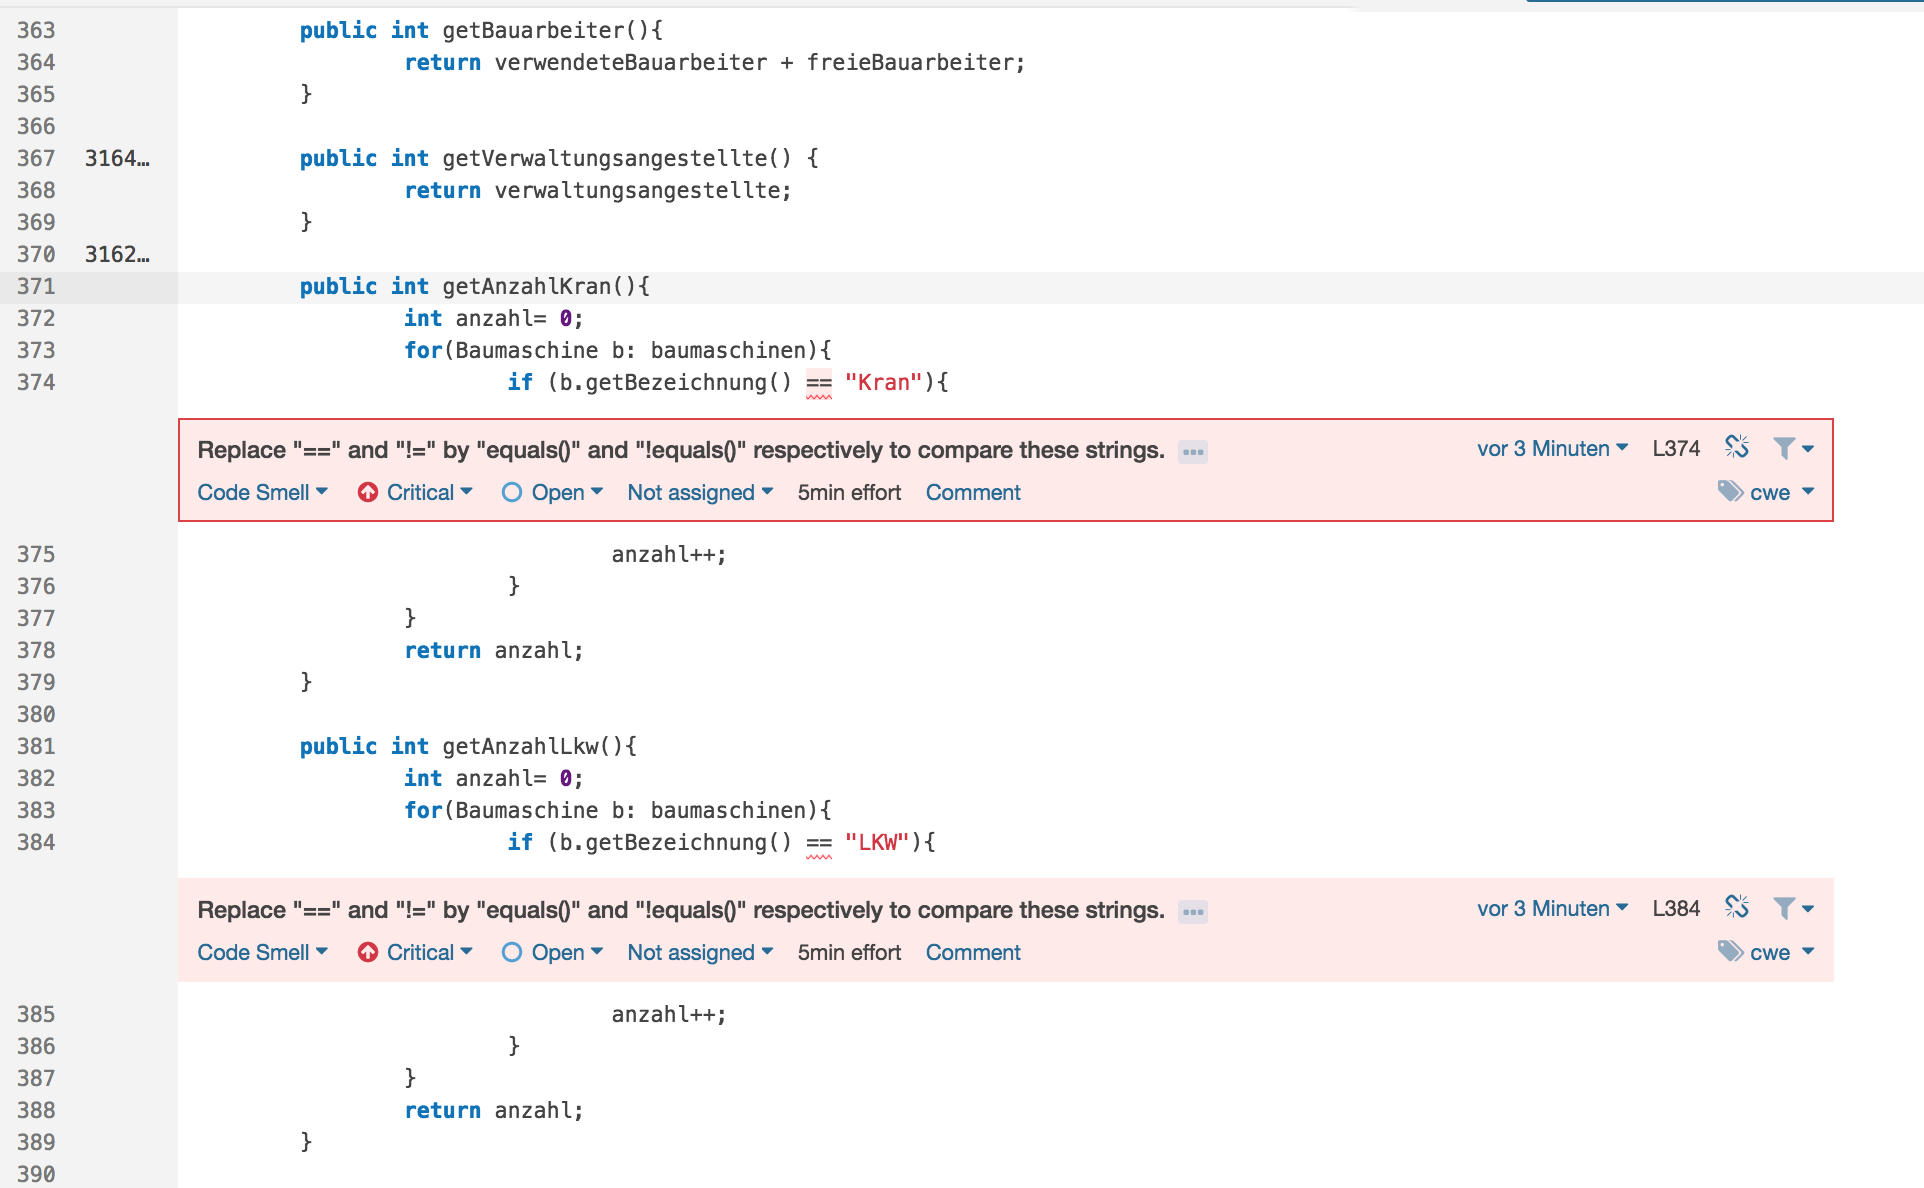
\includegraphics[scale=0.45]{img/fehlerSonar}
	\captionof{figure}{\label{abb:fehlersonar}Sonar entdeckt das Verwenden eines doppelten Gleichzeichens statt eines equals-Ausdruck.}
	\vspace{2em}
\end{minipage}
